\section{Theorie}
\label{sec:Theorie}

% In knapper Form sind die physikalischen Grundlagen des Versuches, des Messverfahrens, sowie sämtliche für die Auswertung erforderlichen Gleichungen darzustellen. (Keine Herleitung)

% (eventuell die Aufgaben)

% Der Versuchsaufbau: Beschreibung des Versuchs und der Funktionsweise (mit Skizze/Bild/Foto)

\subsection{Funktionsweise und Aufbau eines Geiger-Müller-Zählrohrs}
\label{ssec:t1}

Der Aufbau eines Geiger-Müller-Zählrohrs ist in \autoref{fig:geiger} dargestellt.
Er besteht aus einem Stahlmantel, der gleichzeitig als Kathode dient. 
Der Mantel hat den Radius $r_\text{K}$.
Im Inneren des Zylinders befindet sich die entsprechende Anode, ein Draht der darin axial verläuft.
Dieser hat den Radius $r_\text{a}$.
Außerdem befindet sich im Innenraum noch ein Gasgemisch.
Die zu messende Strahlung muss ein Fenster aus Mylar passieren, dieses ist dünn genug um selbst $\alpha$-Strahlung hindurch zulassen.

\begin{figure}
    \centering
    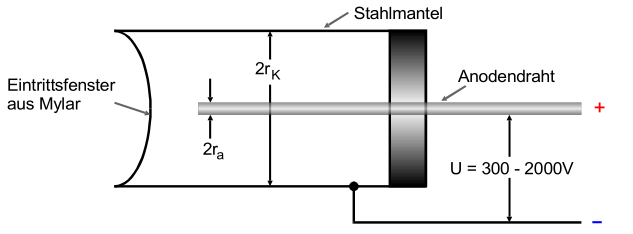
\includegraphics[width=\textwidth]{images/bild2.png}
    \caption{Aufbau eines Geiger-Müller-Zählrohrs}
    \label{fig:geiger}
\end{figure}

Nun kann eine äußere Spannung $U$ angelegt werden, diese liegt typischerweise zwischen $300$ und $\SI{2000}{\volt}$.
Dadurch einsteht zwischen Draht und Mantel ein radialsymmetrisches Feld mit der Feldstärke 

\begin{equation}
    E = \frac{U}{r \cdot \ln{\frac{r_\text{K}}{r_\text{a}}}}.
    \label{eq:energie}
\end{equation}


Trifft nun ein Teilchen durch das Fenster in das Zählrohr wird es zwangsläufig seine Energie an Ionisationsprozesse verlieren.
Das bedeutet, es spaltet Verbindungen, sodass danach Elektronen und positive Ionen entstehen.
Die danach ablaufenden Prozesse sind stark abhängig von der angelegten Spannung $U$, diese Abhängigkeit ist in \autoref{fig:paare} dargestellt.

\begin{figure}
    \centering
    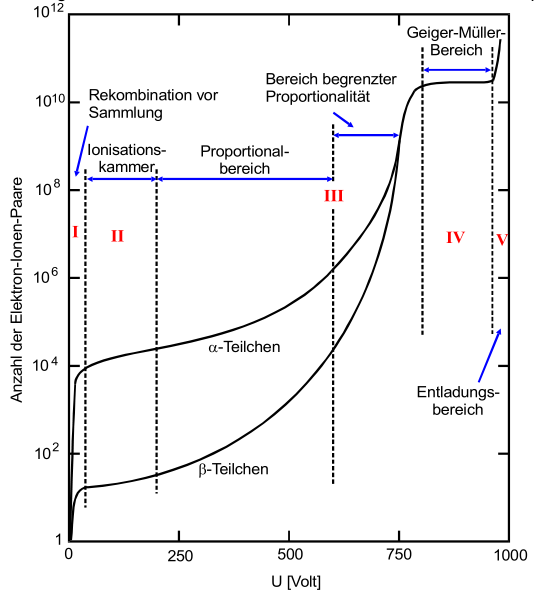
\includegraphics[width=\textwidth]{images/bild3.png}
    \caption{Abhängigkeit der gebildeten Paare von der Spannung}
    \label{fig:paare}
\end{figure}

In Sektion I ist die Spannung nicht groß genug, werden die Elektronen nicht schnell genug zum Anodendraht bewegt und sie verlieren ihre gesamte Enerige in Folge von Rekombinationsprozessen.
Wird die Spannung erhöht verschiwndet dieses Problem immer mehr und die Elektronen erreichen fast alle den Draht.
Wichtig ist hier, dass der Ionisationsstrom in Bereich II zwischen Anode und Kathode proportional zur Intensität der einfallenden Strahlung ist.
Geräte die in diesem Bereich betrieben werden, werden als Ionisationskammern bezeichnet, einer Vorstufe des Geiger-Müller Zählers.
Nach erneuter Erhöhung des Stroms erreichen die Elektronen Energie, die hoch genug sind um selber in Stoßprozessen neue Elektronen-Ionen Paare zu bilden. 
Die in diesen Stoßionisation gebildeten Elektronen sind ihrerseits auch wieder energetisch genug um weitere Paare zu bilden.
Eine solche Welle an Paarbildungen wird auch Townsend-Lawine genannt.
Auch in diesem Bereich ist die Enerige noch proportional zu der Ladung $Q$ ist, kann dadurch die Teilchenenergie bestimmt werden.
Im Bereich IV arbeitet das Geiger-Müller-Zählrohr.
Die Proportionalität geht verloren, die Elektronen setzen bei ihren Zusammenstößen zusätzlich Photonen frei, die sich unabhängnig vom Elektrischen Feld bewegen können. 
Es treten überall Ionisationen auf und die Gesamtladung $Q$ hängt schließlich nur noch vom Volumen des Zylinders ab. Nun kann das Zählrohr nur noch die Intensitäten messen.

\subsection{Charakteristik}
\label{ssec:t2}

Wird bei konstanter Strahlenintensität die Anzahl der gemessenen Impulse gegen die Spannung aufgetragen entsteht ein Bild wie in \autoref{fig:charakteristik}.

\begin{figure}
    \centering
    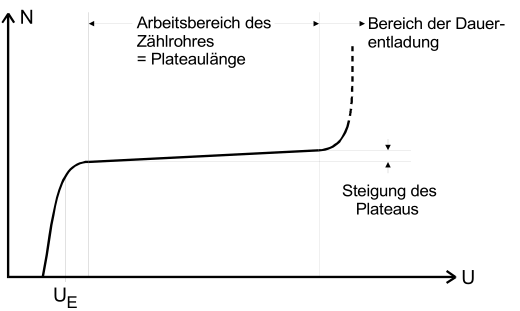
\includegraphics[width=\textwidth]{images/bild4.png}
    \caption{Charakteristik eines Zählrohrs bei konstanter Intensität}
    \label{fig:charakteristik}
\end{figure}

Dieses Bild wird Charakteristik genannt und stellt grob die Abhängigkeit in Bereich V aus \autoref{fig:paare} dar.
An den Bereich III schließt sich hier der Arbeitsbereich des Geiger-Müller-Zählrohres an.
Der Arbeitsbereich wird Plateau genannt und sollte im optimalen Fall keine Steigung besitzen.
Aufgrund von unerwünschten Nachentladungen wird diese aber nie null sein, das bedeutet eine optimales Zählrohr hat in diesem Bereich keine Steigung.

\subsection{Totzeit}
\label{ssec:t3}

Die sogenannte Totzeit $\tau$ kommt durch die bei den Paarbildungen entstandenen positiven Ionen.
Aufgrund der Coulomb-Anziehung bewegen sie sich zum Zylindermantel, sie sind allerdings viel träger als die Elektronen und in der Zeit senken sie mit ihrer Ladung das E-Feld herab.
Das bedeutet die Elektronen sind unter Umständen erneut zu langsam, wie in Bereich I in \autoref{ssec:t1} und gehen an den Ionisationen zugrunde. 
Es würden also Impulse verloren gehen.
Ist diese Totzeit bekannt, ist es möglich sie zu korrigieren.
Dafür kann die Zwei-Quellen-Methode genutzt werden.
Es werden die Intensitäten zweier Quellen gemessen.
Schließlich werden die Intensitäten beider Quellen zusammen gemessen, über 

\begin{equation}
    \frac{N_\text{1+2}}{1 - \tau \cdot N_\text{1+2}} = \frac{N_\text{1}}{1 - \tau \cdot N_\text{1}} + \frac{N_\text{2}}{1 - \tau \cdot N_\text{2}}
    \label{eq:tot1}
\end{equation}

kann dann die Totzeit bestimmt werden.
Falls für alle Intensitäten gilt $\tau ^2 \cdot N^2 << 1$ kann $\tau$ über 

\begin{equation}
    \tau = \frac{N_\text{1} + N_\text{2} - N_\text{1+2}}{2 N_\text{1} N_\text{2}}
    \label{eq:tot2}
\end{equation}

bestimmt werden.

\subsection{Zahl der freigesetzte Ladungen pro einfallendem Teilchen}
\label{ssec:t4}

Mit der mittleren Zählrohrstrom $I$ und der Intensität $N$ kann die Anzahl der freigesetzten Ladungen pro einfallendem Teilchen 

\begin{equation}
    Z = \frac{I}{e_0 \cdot N} 
    \label{eq:z}
\end{equation}

berechnet werden, dabei ist $e_0$ die Elektronenladung.